\documentclass[a4paper]{article}
\usepackage[margin=2.5cm]{geometry}
\usepackage{amsmath}
\usepackage{booktabs}
\usepackage{graphicx}
\usepackage{color}
\usepackage{setspace}
  \onehalfspacing
\usepackage{float}
%\usepackage{mathpazo}

\renewcommand{\textfraction}{0.05}
\renewcommand{\topfraction}{0.95}
\renewcommand{\bottomfraction}{0.95}
\renewcommand{\floatpagefraction}{0.35}
\setcounter{totalnumber}{5}

\title{Sensitivity behaviour of the reliability index against initiation of 
       supercritical flow in triangular channels
      }
\author{Mohanadas Harish Chandar, U067314J}

\begin{document}
\maketitle

\section{Summary}
Flow in open channels can be classified as subcritical or supercritical.
For the same flow rate, subcritical flow is characterised by a higher water 
depth and lower water velocity than supercritical flow.
In practice, it is often desirable to ensure that the flow remains within the 
subcritical range. This may be for reasons such as to control flow
from downstream locations, to ensure smooth uniform flow under conditions
of varying channel bottom slopes, or to keep velocity low so as to reduce
erosion.

In this study, the sensitivity of the reliability index against
initiation of supercritical flow was investigated in triangular sections.
The FORM method of reliability analysis was adopted in the calculation
of reliability indexes, and a verification study was conducted 
for a subset of the results using Monte Carlo simulations.

At the end of the study, the results and findings were compared to 
norms in civil engineering practice and back-compared to the performance function
so as to make design recommedations.

\section{Objectives and scope}
The objectives of the study were to qualitatively investigate the 
sensitivity of the reliability index under variations in

\begin{itemize}
\item Channel bed slope, $S$
\item Manning's roughness coefficient, $n$
\item Flow rate, $Q$
\item Section slope, $m$
\end{itemize}

so that design recommendations could be made.

To keep the mathematics simple, only triangular sections were analyzed in the 
current study. $m$ was taken to be the ratio between the horizontal distance to
the vertical distance of the side walls in the triangular sections.

Four different sections (A--D) were investigated in the study. The baseline
mean values for the parameters of each section are given in Table~\ref{tab:x_b},
where $\bar{X_b}$ refers to the baseline mean value of parameter $X$.
The value of $\bar{S_b}$ = 0.00100 corresponded to a 1\,m drop in elevation for every 1\,km
in channel length and the value of $\bar{n_b}$ = 0.0120 corresponded to that of smooth concrete.
For each channel section, $\bar{Q_b}$ was set to the value which resulted in a reliability index of 
$\beta=2.5$ for that section.

\begin{table}[htbp]
\centering
\begin{tabular}{cccccc} \toprule
Section & \multicolumn{1}{c}{$\bar{m_b}$} & \multicolumn{1}{c}{$\bar{S_b}$} & \multicolumn{1}{c}{$\bar{n_b}$} & \multicolumn{1}{c}{$\bar{Q_b}$} & \multicolumn{1}{c}{$\beta_b$} \\ \midrule
A & 0.75 & 0.00100 & 0.0120 & 250 & 2.5 \\ 
B & 1.0 & 0.00100 & 0.0120 & 67.5 & 2.5 \\ 
C & 1.5 & 0.00100 & 0.0120 & 20 & 2.5 \\ 
D & 2.0 & 0.00100 & 0.0120 & 12 & 2.5 \\ \bottomrule
\end{tabular}
\caption{Baseline mean values of variables under investigation. 
         $\bar{X_b}$ refers to the baseline mean value of parameter $X$.}
\label{tab:x_b}
\end{table}



\newpage
\section{Theory/method}
The performance function for the investigation was given by

\begin{align*}
g(\mathbf{X}) &= y - y_c \\
              &= 4^{1/8}Q^{3/8}n^{3/8}m^{-5/8}(1+m)^{1/8}S^{-3/16} - 2^{1/5}Q^{2/5}m^{-2/5}g^{-1/5}
\end{align*}
where $y$ = flow depth; $y_c$ = critical flow depth; and $g$ = acceleration due to gravity.

The reliability indexes of the various scenarios was determined through FORM.
In particular, the gradient projection method of FORM was used to calculate the 
reliability index values.
Monte Carlo simulations (with 50,000 trials each) 
were used for verification of a subset of the results.

In this study, all the parameters under investigation ($S$, $n$, $Q$ and $m$) 
were assumed to normally distributed with a constant coefficient of variation 
as given in Table~\ref{tab:cov}.
$g$ was taken to be constant at 9.81\,m/s.
Only the mean values of the variables under investigation were varied.
The range of variation in the mean values was chosen to roughly 
cover a reliability index range of $1 \leq \beta \leq 4$ for each investigation.

\begin{table}[htbp]
\centering
\begin{tabular}{lllll} \toprule
 & \multicolumn{1}{c}{$m$} & \multicolumn{1}{c}{$S$} & \multicolumn{1}{c}{$n$} & \multicolumn{1}{c}{$Q$}\\ \midrule
\multicolumn{1}{c}{COV} & \multicolumn{1}{r}{0.01} & \multicolumn{1}{r}{0.05} & \multicolumn{1}{r}{0.1} & \multicolumn{1}{r}{0.2} \\ \bottomrule
\end{tabular}
\caption{Coefficient of variation of variables under investigation.}
\label{tab:cov}
\end{table}



\section{Results}
\subsection{Verification study}
\begin{figure}[H]
\centering
% GNUPLOT: LaTeX picture with Postscript
\begingroup
  \makeatletter
  \providecommand\color[2][]{%
    \GenericError{(gnuplot) \space\space\space\@spaces}{%
      Package color not loaded in conjunction with
      terminal option `colourtext'%
    }{See the gnuplot documentation for explanation.%
    }{Either use 'blacktext' in gnuplot or load the package
      color.sty in LaTeX.}%
    \renewcommand\color[2][]{}%
  }%
  \providecommand\includegraphics[2][]{%
    \GenericError{(gnuplot) \space\space\space\@spaces}{%
      Package graphicx or graphics not loaded%
    }{See the gnuplot documentation for explanation.%
    }{The gnuplot epslatex terminal needs graphicx.sty or graphics.sty.}%
    \renewcommand\includegraphics[2][]{}%
  }%
  \providecommand\rotatebox[2]{#2}%
  \@ifundefined{ifGPcolor}{%
    \newif\ifGPcolor
    \GPcolortrue
  }{}%
  \@ifundefined{ifGPblacktext}{%
    \newif\ifGPblacktext
    \GPblacktexttrue
  }{}%
  % define a \g@addto@macro without @ in the name:
  \let\gplgaddtomacro\g@addto@macro
  % define empty templates for all commands taking text:
  \gdef\gplbacktext{}%
  \gdef\gplfronttext{}%
  \makeatother
  \ifGPblacktext
    % no textcolor at all
    \def\colorrgb#1{}%
    \def\colorgray#1{}%
  \else
    % gray or color?
    \ifGPcolor
      \def\colorrgb#1{\color[rgb]{#1}}%
      \def\colorgray#1{\color[gray]{#1}}%
      \expandafter\def\csname LTw\endcsname{\color{white}}%
      \expandafter\def\csname LTb\endcsname{\color{black}}%
      \expandafter\def\csname LTa\endcsname{\color{black}}%
      \expandafter\def\csname LT0\endcsname{\color[rgb]{1,0,0}}%
      \expandafter\def\csname LT1\endcsname{\color[rgb]{0,1,0}}%
      \expandafter\def\csname LT2\endcsname{\color[rgb]{0,0,1}}%
      \expandafter\def\csname LT3\endcsname{\color[rgb]{1,0,1}}%
      \expandafter\def\csname LT4\endcsname{\color[rgb]{0,1,1}}%
      \expandafter\def\csname LT5\endcsname{\color[rgb]{1,1,0}}%
      \expandafter\def\csname LT6\endcsname{\color[rgb]{0,0,0}}%
      \expandafter\def\csname LT7\endcsname{\color[rgb]{1,0.3,0}}%
      \expandafter\def\csname LT8\endcsname{\color[rgb]{0.5,0.5,0.5}}%
    \else
      % gray
      \def\colorrgb#1{\color{black}}%
      \def\colorgray#1{\color[gray]{#1}}%
      \expandafter\def\csname LTw\endcsname{\color{white}}%
      \expandafter\def\csname LTb\endcsname{\color{black}}%
      \expandafter\def\csname LTa\endcsname{\color{black}}%
      \expandafter\def\csname LT0\endcsname{\color{black}}%
      \expandafter\def\csname LT1\endcsname{\color{black}}%
      \expandafter\def\csname LT2\endcsname{\color{black}}%
      \expandafter\def\csname LT3\endcsname{\color{black}}%
      \expandafter\def\csname LT4\endcsname{\color{black}}%
      \expandafter\def\csname LT5\endcsname{\color{black}}%
      \expandafter\def\csname LT6\endcsname{\color{black}}%
      \expandafter\def\csname LT7\endcsname{\color{black}}%
      \expandafter\def\csname LT8\endcsname{\color{black}}%
    \fi
  \fi
  \setlength{\unitlength}{0.0500bp}%
  \begin{picture}(7200.00,5040.00)%
    \gplgaddtomacro\gplbacktext{%
      \csname LTb\endcsname%
      \put(1122,704){\makebox(0,0)[r]{\strut{}$0.5$}}%
      \put(1122,1156){\makebox(0,0)[r]{\strut{}$1$}}%
      \put(1122,1609){\makebox(0,0)[r]{\strut{}$1.5$}}%
      \put(1122,2061){\makebox(0,0)[r]{\strut{}$2$}}%
      \put(1122,2514){\makebox(0,0)[r]{\strut{}$2.5$}}%
      \put(1122,2966){\makebox(0,0)[r]{\strut{}$3$}}%
      \put(1122,3419){\makebox(0,0)[r]{\strut{}$3.5$}}%
      \put(1122,3871){\makebox(0,0)[r]{\strut{}$4$}}%
      \put(1122,4324){\makebox(0,0)[r]{\strut{}$4.5$}}%
      \put(1122,4776){\makebox(0,0)[r]{\strut{}$5$}}%
      \put(1254,484){\makebox(0,0){\strut{}$0.00040$}}%
      \put(2190,484){\makebox(0,0){\strut{}$0.00060$}}%
      \put(3126,484){\makebox(0,0){\strut{}$0.00080$}}%
      \put(4062,484){\makebox(0,0){\strut{}$0.00100$}}%
      \put(4998,484){\makebox(0,0){\strut{}$0.00120$}}%
      \put(5934,484){\makebox(0,0){\strut{}$0.00140$}}%
      \put(6870,484){\makebox(0,0){\strut{}$0.00160$}}%
      \put(484,2740){\rotatebox{90}{\makebox(0,0){\strut{}$\beta$}}}%
      \put(4062,154){\makebox(0,0){\strut{}$\bar{S}$}}%
    }%
    \gplgaddtomacro\gplfronttext{%
      \csname LTb\endcsname%
      \put(5883,4603){\makebox(0,0)[r]{\strut{}Section B FORM}}%
      \csname LTb\endcsname%
      \put(5883,4383){\makebox(0,0)[r]{\strut{}Section B Monte Carlo}}%
    }%
    \gplbacktext
    \put(0,0){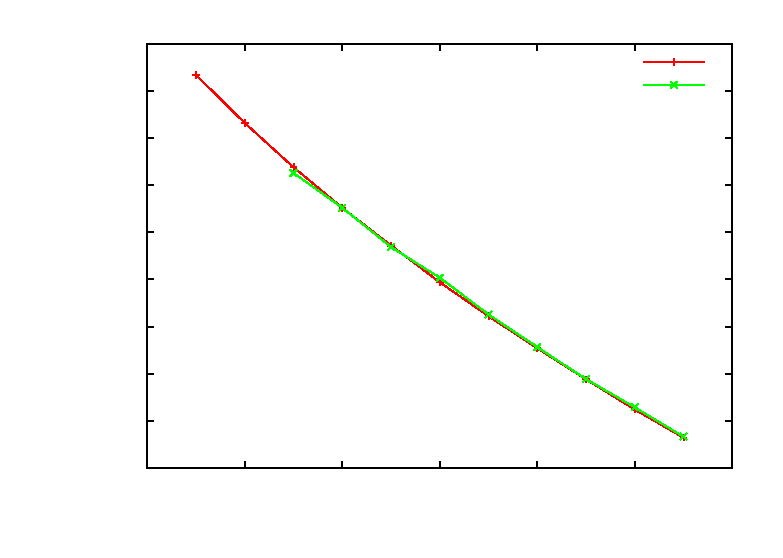
\includegraphics{verification_s}}%
    \gplfronttext
  \end{picture}%
\endgroup

\caption{Plot of verification study on results from variations in channel bed slope for Section B.
         There was good agreement between results from FORM and Monte Carlo simulations.}
\label{fig:verification_s}
\end{figure}

\begin{figure}[H]
\centering
% GNUPLOT: LaTeX picture with Postscript
\begingroup
  \makeatletter
  \providecommand\color[2][]{%
    \GenericError{(gnuplot) \space\space\space\@spaces}{%
      Package color not loaded in conjunction with
      terminal option `colourtext'%
    }{See the gnuplot documentation for explanation.%
    }{Either use 'blacktext' in gnuplot or load the package
      color.sty in LaTeX.}%
    \renewcommand\color[2][]{}%
  }%
  \providecommand\includegraphics[2][]{%
    \GenericError{(gnuplot) \space\space\space\@spaces}{%
      Package graphicx or graphics not loaded%
    }{See the gnuplot documentation for explanation.%
    }{The gnuplot epslatex terminal needs graphicx.sty or graphics.sty.}%
    \renewcommand\includegraphics[2][]{}%
  }%
  \providecommand\rotatebox[2]{#2}%
  \@ifundefined{ifGPcolor}{%
    \newif\ifGPcolor
    \GPcolortrue
  }{}%
  \@ifundefined{ifGPblacktext}{%
    \newif\ifGPblacktext
    \GPblacktexttrue
  }{}%
  % define a \g@addto@macro without @ in the name:
  \let\gplgaddtomacro\g@addto@macro
  % define empty templates for all commands taking text:
  \gdef\gplbacktext{}%
  \gdef\gplfronttext{}%
  \makeatother
  \ifGPblacktext
    % no textcolor at all
    \def\colorrgb#1{}%
    \def\colorgray#1{}%
  \else
    % gray or color?
    \ifGPcolor
      \def\colorrgb#1{\color[rgb]{#1}}%
      \def\colorgray#1{\color[gray]{#1}}%
      \expandafter\def\csname LTw\endcsname{\color{white}}%
      \expandafter\def\csname LTb\endcsname{\color{black}}%
      \expandafter\def\csname LTa\endcsname{\color{black}}%
      \expandafter\def\csname LT0\endcsname{\color[rgb]{1,0,0}}%
      \expandafter\def\csname LT1\endcsname{\color[rgb]{0,1,0}}%
      \expandafter\def\csname LT2\endcsname{\color[rgb]{0,0,1}}%
      \expandafter\def\csname LT3\endcsname{\color[rgb]{1,0,1}}%
      \expandafter\def\csname LT4\endcsname{\color[rgb]{0,1,1}}%
      \expandafter\def\csname LT5\endcsname{\color[rgb]{1,1,0}}%
      \expandafter\def\csname LT6\endcsname{\color[rgb]{0,0,0}}%
      \expandafter\def\csname LT7\endcsname{\color[rgb]{1,0.3,0}}%
      \expandafter\def\csname LT8\endcsname{\color[rgb]{0.5,0.5,0.5}}%
    \else
      % gray
      \def\colorrgb#1{\color{black}}%
      \def\colorgray#1{\color[gray]{#1}}%
      \expandafter\def\csname LTw\endcsname{\color{white}}%
      \expandafter\def\csname LTb\endcsname{\color{black}}%
      \expandafter\def\csname LTa\endcsname{\color{black}}%
      \expandafter\def\csname LT0\endcsname{\color{black}}%
      \expandafter\def\csname LT1\endcsname{\color{black}}%
      \expandafter\def\csname LT2\endcsname{\color{black}}%
      \expandafter\def\csname LT3\endcsname{\color{black}}%
      \expandafter\def\csname LT4\endcsname{\color{black}}%
      \expandafter\def\csname LT5\endcsname{\color{black}}%
      \expandafter\def\csname LT6\endcsname{\color{black}}%
      \expandafter\def\csname LT7\endcsname{\color{black}}%
      \expandafter\def\csname LT8\endcsname{\color{black}}%
    \fi
  \fi
  \setlength{\unitlength}{0.0500bp}%
  \begin{picture}(7200.00,5040.00)%
    \gplgaddtomacro\gplbacktext{%
      \csname LTb\endcsname%
      \put(1122,704){\makebox(0,0)[r]{\strut{}$2$}}%
      \put(1122,1518){\makebox(0,0)[r]{\strut{}$2.2$}}%
      \put(1122,2333){\makebox(0,0)[r]{\strut{}$2.4$}}%
      \put(1122,3147){\makebox(0,0)[r]{\strut{}$2.6$}}%
      \put(1122,3962){\makebox(0,0)[r]{\strut{}$2.8$}}%
      \put(1122,4776){\makebox(0,0)[r]{\strut{}$3$}}%
      \put(1254,484){\makebox(0,0){\strut{}$0.6$}}%
      \put(1878,484){\makebox(0,0){\strut{}$0.7$}}%
      \put(2502,484){\makebox(0,0){\strut{}$0.8$}}%
      \put(3126,484){\makebox(0,0){\strut{}$0.9$}}%
      \put(3750,484){\makebox(0,0){\strut{}$1$}}%
      \put(4374,484){\makebox(0,0){\strut{}$1.1$}}%
      \put(4998,484){\makebox(0,0){\strut{}$1.2$}}%
      \put(5622,484){\makebox(0,0){\strut{}$1.3$}}%
      \put(6246,484){\makebox(0,0){\strut{}$1.4$}}%
      \put(6870,484){\makebox(0,0){\strut{}$1.5$}}%
      \put(484,2740){\rotatebox{90}{\makebox(0,0){\strut{}$\beta$}}}%
      \put(4062,154){\makebox(0,0){\strut{}$\bar{m}/\bar{m_b}$}}%
    }%
    \gplgaddtomacro\gplfronttext{%
      \csname LTb\endcsname%
      \put(5883,4603){\makebox(0,0)[r]{\strut{}Section D FORM}}%
      \csname LTb\endcsname%
      \put(5883,4383){\makebox(0,0)[r]{\strut{}Section D Monte Carlo}}%
    }%
    \gplbacktext
    \put(0,0){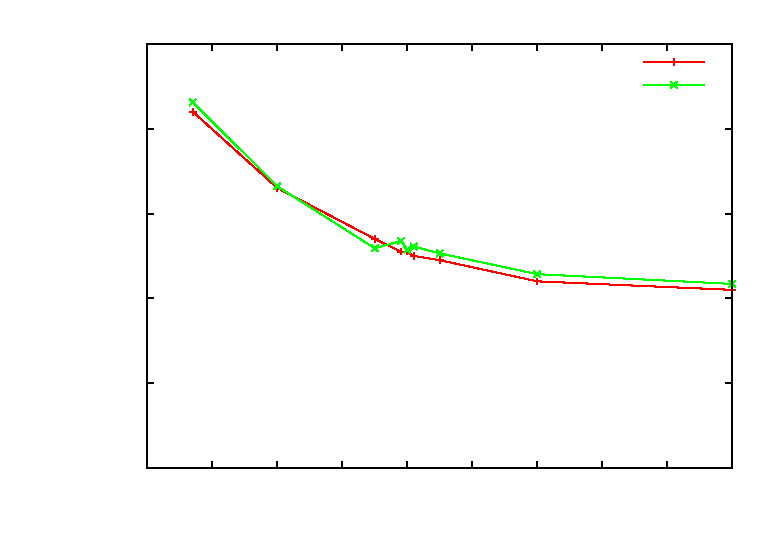
\includegraphics{verification_m}}%
    \gplfronttext
  \end{picture}%
\endgroup

\caption{Plot of verification study on results from variations in section slope for Section D.
         There was good agreement between results from FORM and Monte Carlo simulations.}
\label{fig:verification_m}
\end{figure}

\subsection{Sensitivity of reliability index to variations in channel bed slope}
\begin{figure}[H]
\centering
% GNUPLOT: LaTeX picture with Postscript
\begingroup
  \makeatletter
  \providecommand\color[2][]{%
    \GenericError{(gnuplot) \space\space\space\@spaces}{%
      Package color not loaded in conjunction with
      terminal option `colourtext'%
    }{See the gnuplot documentation for explanation.%
    }{Either use 'blacktext' in gnuplot or load the package
      color.sty in LaTeX.}%
    \renewcommand\color[2][]{}%
  }%
  \providecommand\includegraphics[2][]{%
    \GenericError{(gnuplot) \space\space\space\@spaces}{%
      Package graphicx or graphics not loaded%
    }{See the gnuplot documentation for explanation.%
    }{The gnuplot epslatex terminal needs graphicx.sty or graphics.sty.}%
    \renewcommand\includegraphics[2][]{}%
  }%
  \providecommand\rotatebox[2]{#2}%
  \@ifundefined{ifGPcolor}{%
    \newif\ifGPcolor
    \GPcolortrue
  }{}%
  \@ifundefined{ifGPblacktext}{%
    \newif\ifGPblacktext
    \GPblacktexttrue
  }{}%
  % define a \g@addto@macro without @ in the name:
  \let\gplgaddtomacro\g@addto@macro
  % define empty templates for all commands taking text:
  \gdef\gplbacktext{}%
  \gdef\gplfronttext{}%
  \makeatother
  \ifGPblacktext
    % no textcolor at all
    \def\colorrgb#1{}%
    \def\colorgray#1{}%
  \else
    % gray or color?
    \ifGPcolor
      \def\colorrgb#1{\color[rgb]{#1}}%
      \def\colorgray#1{\color[gray]{#1}}%
      \expandafter\def\csname LTw\endcsname{\color{white}}%
      \expandafter\def\csname LTb\endcsname{\color{black}}%
      \expandafter\def\csname LTa\endcsname{\color{black}}%
      \expandafter\def\csname LT0\endcsname{\color[rgb]{1,0,0}}%
      \expandafter\def\csname LT1\endcsname{\color[rgb]{0,1,0}}%
      \expandafter\def\csname LT2\endcsname{\color[rgb]{0,0,1}}%
      \expandafter\def\csname LT3\endcsname{\color[rgb]{1,0,1}}%
      \expandafter\def\csname LT4\endcsname{\color[rgb]{0,1,1}}%
      \expandafter\def\csname LT5\endcsname{\color[rgb]{1,1,0}}%
      \expandafter\def\csname LT6\endcsname{\color[rgb]{0,0,0}}%
      \expandafter\def\csname LT7\endcsname{\color[rgb]{1,0.3,0}}%
      \expandafter\def\csname LT8\endcsname{\color[rgb]{0.5,0.5,0.5}}%
    \else
      % gray
      \def\colorrgb#1{\color{black}}%
      \def\colorgray#1{\color[gray]{#1}}%
      \expandafter\def\csname LTw\endcsname{\color{white}}%
      \expandafter\def\csname LTb\endcsname{\color{black}}%
      \expandafter\def\csname LTa\endcsname{\color{black}}%
      \expandafter\def\csname LT0\endcsname{\color{black}}%
      \expandafter\def\csname LT1\endcsname{\color{black}}%
      \expandafter\def\csname LT2\endcsname{\color{black}}%
      \expandafter\def\csname LT3\endcsname{\color{black}}%
      \expandafter\def\csname LT4\endcsname{\color{black}}%
      \expandafter\def\csname LT5\endcsname{\color{black}}%
      \expandafter\def\csname LT6\endcsname{\color{black}}%
      \expandafter\def\csname LT7\endcsname{\color{black}}%
      \expandafter\def\csname LT8\endcsname{\color{black}}%
    \fi
  \fi
  \setlength{\unitlength}{0.0500bp}%
  \begin{picture}(7200.00,5040.00)%
    \gplgaddtomacro\gplbacktext{%
      \csname LTb\endcsname%
      \put(1078,704){\makebox(0,0)[r]{\strut{}$0$}}%
      \put(1078,1518){\makebox(0,0)[r]{\strut{}$1$}}%
      \put(1078,2333){\makebox(0,0)[r]{\strut{}$2$}}%
      \put(1078,3147){\makebox(0,0)[r]{\strut{}$3$}}%
      \put(1078,3962){\makebox(0,0)[r]{\strut{}$4$}}%
      \put(1078,4776){\makebox(0,0)[r]{\strut{}$5$}}%
      \put(1210,484){\makebox(0,0){\strut{}$0.00040$}}%
      \put(2153,484){\makebox(0,0){\strut{}$0.00060$}}%
      \put(3097,484){\makebox(0,0){\strut{}$0.00080$}}%
      \put(4040,484){\makebox(0,0){\strut{}$0.00100$}}%
      \put(4983,484){\makebox(0,0){\strut{}$0.00120$}}%
      \put(5927,484){\makebox(0,0){\strut{}$0.00140$}}%
      \put(6870,484){\makebox(0,0){\strut{}$0.00160$}}%
      \put(440,2740){\rotatebox{90}{\makebox(0,0){\strut{}$\beta$}}}%
      \put(4040,154){\makebox(0,0){\strut{}$\bar{S}$}}%
    }%
    \gplgaddtomacro\gplfronttext{%
      \csname LTb\endcsname%
      \put(5883,4603){\makebox(0,0)[r]{\strut{}Section A}}%
      \csname LTb\endcsname%
      \put(5883,4383){\makebox(0,0)[r]{\strut{}Section B}}%
      \csname LTb\endcsname%
      \put(5883,4163){\makebox(0,0)[r]{\strut{}Section C}}%
      \csname LTb\endcsname%
      \put(5883,3943){\makebox(0,0)[r]{\strut{}Section D}}%
    }%
    \gplbacktext
    \put(0,0){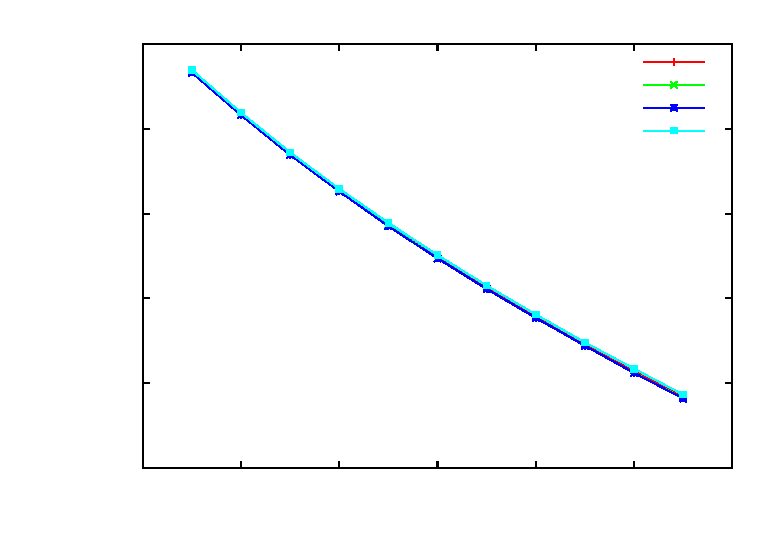
\includegraphics{vary_s}}%
    \gplfronttext
  \end{picture}%
\endgroup

\caption{Plot of reliability index versus channel bed slope for all sections.
         All sections showed very similar responses.}
\label{fig:vary_s}
\end{figure}

\subsection{Sensitivity of reliability index to variations in Manning's roughness coefficient}
\begin{figure}[H]
\centering
% GNUPLOT: LaTeX picture with Postscript
\begingroup
  \makeatletter
  \providecommand\color[2][]{%
    \GenericError{(gnuplot) \space\space\space\@spaces}{%
      Package color not loaded in conjunction with
      terminal option `colourtext'%
    }{See the gnuplot documentation for explanation.%
    }{Either use 'blacktext' in gnuplot or load the package
      color.sty in LaTeX.}%
    \renewcommand\color[2][]{}%
  }%
  \providecommand\includegraphics[2][]{%
    \GenericError{(gnuplot) \space\space\space\@spaces}{%
      Package graphicx or graphics not loaded%
    }{See the gnuplot documentation for explanation.%
    }{The gnuplot epslatex terminal needs graphicx.sty or graphics.sty.}%
    \renewcommand\includegraphics[2][]{}%
  }%
  \providecommand\rotatebox[2]{#2}%
  \@ifundefined{ifGPcolor}{%
    \newif\ifGPcolor
    \GPcolortrue
  }{}%
  \@ifundefined{ifGPblacktext}{%
    \newif\ifGPblacktext
    \GPblacktexttrue
  }{}%
  % define a \g@addto@macro without @ in the name:
  \let\gplgaddtomacro\g@addto@macro
  % define empty templates for all commands taking text:
  \gdef\gplbacktext{}%
  \gdef\gplfronttext{}%
  \makeatother
  \ifGPblacktext
    % no textcolor at all
    \def\colorrgb#1{}%
    \def\colorgray#1{}%
  \else
    % gray or color?
    \ifGPcolor
      \def\colorrgb#1{\color[rgb]{#1}}%
      \def\colorgray#1{\color[gray]{#1}}%
      \expandafter\def\csname LTw\endcsname{\color{white}}%
      \expandafter\def\csname LTb\endcsname{\color{black}}%
      \expandafter\def\csname LTa\endcsname{\color{black}}%
      \expandafter\def\csname LT0\endcsname{\color[rgb]{1,0,0}}%
      \expandafter\def\csname LT1\endcsname{\color[rgb]{0,1,0}}%
      \expandafter\def\csname LT2\endcsname{\color[rgb]{0,0,1}}%
      \expandafter\def\csname LT3\endcsname{\color[rgb]{1,0,1}}%
      \expandafter\def\csname LT4\endcsname{\color[rgb]{0,1,1}}%
      \expandafter\def\csname LT5\endcsname{\color[rgb]{1,1,0}}%
      \expandafter\def\csname LT6\endcsname{\color[rgb]{0,0,0}}%
      \expandafter\def\csname LT7\endcsname{\color[rgb]{1,0.3,0}}%
      \expandafter\def\csname LT8\endcsname{\color[rgb]{0.5,0.5,0.5}}%
    \else
      % gray
      \def\colorrgb#1{\color{black}}%
      \def\colorgray#1{\color[gray]{#1}}%
      \expandafter\def\csname LTw\endcsname{\color{white}}%
      \expandafter\def\csname LTb\endcsname{\color{black}}%
      \expandafter\def\csname LTa\endcsname{\color{black}}%
      \expandafter\def\csname LT0\endcsname{\color{black}}%
      \expandafter\def\csname LT1\endcsname{\color{black}}%
      \expandafter\def\csname LT2\endcsname{\color{black}}%
      \expandafter\def\csname LT3\endcsname{\color{black}}%
      \expandafter\def\csname LT4\endcsname{\color{black}}%
      \expandafter\def\csname LT5\endcsname{\color{black}}%
      \expandafter\def\csname LT6\endcsname{\color{black}}%
      \expandafter\def\csname LT7\endcsname{\color{black}}%
      \expandafter\def\csname LT8\endcsname{\color{black}}%
    \fi
  \fi
  \setlength{\unitlength}{0.0500bp}%
  \begin{picture}(7200.00,5040.00)%
    \gplgaddtomacro\gplbacktext{%
      \csname LTb\endcsname%
      \put(858,704){\makebox(0,0)[r]{\strut{}$0$}}%
      \put(858,1518){\makebox(0,0)[r]{\strut{}$1$}}%
      \put(858,2333){\makebox(0,0)[r]{\strut{}$2$}}%
      \put(858,3147){\makebox(0,0)[r]{\strut{}$3$}}%
      \put(858,3962){\makebox(0,0)[r]{\strut{}$4$}}%
      \put(858,4776){\makebox(0,0)[r]{\strut{}$5$}}%
      \put(990,484){\makebox(0,0){\strut{}$0.009$}}%
      \put(1830,484){\makebox(0,0){\strut{}$0.010$}}%
      \put(2670,484){\makebox(0,0){\strut{}$0.011$}}%
      \put(3510,484){\makebox(0,0){\strut{}$0.012$}}%
      \put(4350,484){\makebox(0,0){\strut{}$0.013$}}%
      \put(5190,484){\makebox(0,0){\strut{}$0.014$}}%
      \put(6030,484){\makebox(0,0){\strut{}$0.015$}}%
      \put(6870,484){\makebox(0,0){\strut{}$0.016$}}%
      \put(484,2740){\rotatebox{90}{\makebox(0,0){\strut{}$\beta$}}}%
      \put(3930,154){\makebox(0,0){\strut{}$\bar{n}$}}%
    }%
    \gplgaddtomacro\gplfronttext{%
      \csname LTb\endcsname%
      \put(5883,4603){\makebox(0,0)[r]{\strut{}Section A}}%
      \csname LTb\endcsname%
      \put(5883,4383){\makebox(0,0)[r]{\strut{}Section B}}%
      \csname LTb\endcsname%
      \put(5883,4163){\makebox(0,0)[r]{\strut{}Section C}}%
      \csname LTb\endcsname%
      \put(5883,3943){\makebox(0,0)[r]{\strut{}Section D}}%
    }%
    \gplbacktext
    \put(0,0){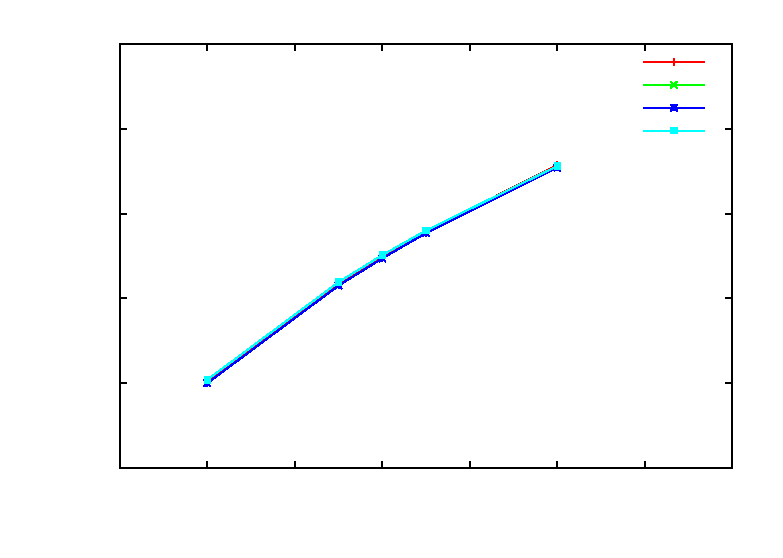
\includegraphics{vary_n}}%
    \gplfronttext
  \end{picture}%
\endgroup

\caption{Plot of reliability index versus Manning's roughness coefficient for all sections.
         All sections showed very similar responses.}
\label{fig:vary_n}
\end{figure}

\subsection{Sensitivity of reliability index to variations in flow rate}
\begin{figure}[H]
\centering
% GNUPLOT: LaTeX picture with Postscript
\begingroup
  \makeatletter
  \providecommand\color[2][]{%
    \GenericError{(gnuplot) \space\space\space\@spaces}{%
      Package color not loaded in conjunction with
      terminal option `colourtext'%
    }{See the gnuplot documentation for explanation.%
    }{Either use 'blacktext' in gnuplot or load the package
      color.sty in LaTeX.}%
    \renewcommand\color[2][]{}%
  }%
  \providecommand\includegraphics[2][]{%
    \GenericError{(gnuplot) \space\space\space\@spaces}{%
      Package graphicx or graphics not loaded%
    }{See the gnuplot documentation for explanation.%
    }{The gnuplot epslatex terminal needs graphicx.sty or graphics.sty.}%
    \renewcommand\includegraphics[2][]{}%
  }%
  \providecommand\rotatebox[2]{#2}%
  \@ifundefined{ifGPcolor}{%
    \newif\ifGPcolor
    \GPcolortrue
  }{}%
  \@ifundefined{ifGPblacktext}{%
    \newif\ifGPblacktext
    \GPblacktexttrue
  }{}%
  % define a \g@addto@macro without @ in the name:
  \let\gplgaddtomacro\g@addto@macro
  % define empty templates for all commands taking text:
  \gdef\gplbacktext{}%
  \gdef\gplfronttext{}%
  \makeatother
  \ifGPblacktext
    % no textcolor at all
    \def\colorrgb#1{}%
    \def\colorgray#1{}%
  \else
    % gray or color?
    \ifGPcolor
      \def\colorrgb#1{\color[rgb]{#1}}%
      \def\colorgray#1{\color[gray]{#1}}%
      \expandafter\def\csname LTw\endcsname{\color{white}}%
      \expandafter\def\csname LTb\endcsname{\color{black}}%
      \expandafter\def\csname LTa\endcsname{\color{black}}%
      \expandafter\def\csname LT0\endcsname{\color[rgb]{1,0,0}}%
      \expandafter\def\csname LT1\endcsname{\color[rgb]{0,1,0}}%
      \expandafter\def\csname LT2\endcsname{\color[rgb]{0,0,1}}%
      \expandafter\def\csname LT3\endcsname{\color[rgb]{1,0,1}}%
      \expandafter\def\csname LT4\endcsname{\color[rgb]{0,1,1}}%
      \expandafter\def\csname LT5\endcsname{\color[rgb]{1,1,0}}%
      \expandafter\def\csname LT6\endcsname{\color[rgb]{0,0,0}}%
      \expandafter\def\csname LT7\endcsname{\color[rgb]{1,0.3,0}}%
      \expandafter\def\csname LT8\endcsname{\color[rgb]{0.5,0.5,0.5}}%
    \else
      % gray
      \def\colorrgb#1{\color{black}}%
      \def\colorgray#1{\color[gray]{#1}}%
      \expandafter\def\csname LTw\endcsname{\color{white}}%
      \expandafter\def\csname LTb\endcsname{\color{black}}%
      \expandafter\def\csname LTa\endcsname{\color{black}}%
      \expandafter\def\csname LT0\endcsname{\color{black}}%
      \expandafter\def\csname LT1\endcsname{\color{black}}%
      \expandafter\def\csname LT2\endcsname{\color{black}}%
      \expandafter\def\csname LT3\endcsname{\color{black}}%
      \expandafter\def\csname LT4\endcsname{\color{black}}%
      \expandafter\def\csname LT5\endcsname{\color{black}}%
      \expandafter\def\csname LT6\endcsname{\color{black}}%
      \expandafter\def\csname LT7\endcsname{\color{black}}%
      \expandafter\def\csname LT8\endcsname{\color{black}}%
    \fi
  \fi
  \setlength{\unitlength}{0.0500bp}%
  \begin{picture}(7200.00,5040.00)%
    \gplgaddtomacro\gplbacktext{%
      \csname LTb\endcsname%
      \put(858,704){\makebox(0,0)[r]{\strut{}$0$}}%
      \put(858,1518){\makebox(0,0)[r]{\strut{}$1$}}%
      \put(858,2333){\makebox(0,0)[r]{\strut{}$2$}}%
      \put(858,3147){\makebox(0,0)[r]{\strut{}$3$}}%
      \put(858,3962){\makebox(0,0)[r]{\strut{}$4$}}%
      \put(858,4776){\makebox(0,0)[r]{\strut{}$5$}}%
      \put(990,484){\makebox(0,0){\strut{}$0$}}%
      \put(1578,484){\makebox(0,0){\strut{}$0.5$}}%
      \put(2166,484){\makebox(0,0){\strut{}$1$}}%
      \put(2754,484){\makebox(0,0){\strut{}$1.5$}}%
      \put(3342,484){\makebox(0,0){\strut{}$2$}}%
      \put(3930,484){\makebox(0,0){\strut{}$2.5$}}%
      \put(4518,484){\makebox(0,0){\strut{}$3$}}%
      \put(5106,484){\makebox(0,0){\strut{}$3.5$}}%
      \put(5694,484){\makebox(0,0){\strut{}$4$}}%
      \put(6282,484){\makebox(0,0){\strut{}$4.5$}}%
      \put(6870,484){\makebox(0,0){\strut{}$5$}}%
      \put(484,2740){\rotatebox{90}{\makebox(0,0){\strut{}$\beta$}}}%
      \put(3930,154){\makebox(0,0){\strut{}$\bar{Q}/\bar{Q_b}$}}%
    }%
    \gplgaddtomacro\gplfronttext{%
      \csname LTb\endcsname%
      \put(5883,4603){\makebox(0,0)[r]{\strut{}Section A}}%
      \csname LTb\endcsname%
      \put(5883,4383){\makebox(0,0)[r]{\strut{}Section B}}%
      \csname LTb\endcsname%
      \put(5883,4163){\makebox(0,0)[r]{\strut{}Section C}}%
      \csname LTb\endcsname%
      \put(5883,3943){\makebox(0,0)[r]{\strut{}Section D}}%
    }%
    \gplbacktext
    \put(0,0){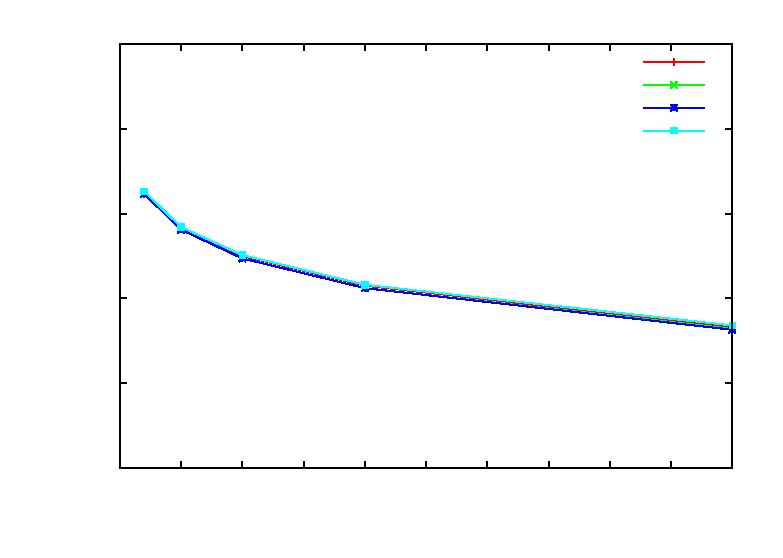
\includegraphics{vary_q}}%
    \gplfronttext
  \end{picture}%
\endgroup

\caption{Plot of reliability index versus flow rate for all sections.
         All sections showed very similar responses.}
\label{fig:vary_q}
\end{figure}

\subsection{Sensitivity of reliability index to variations in section slope}
\begin{figure}[H]
\centering
% GNUPLOT: LaTeX picture with Postscript
\begingroup
  \makeatletter
  \providecommand\color[2][]{%
    \GenericError{(gnuplot) \space\space\space\@spaces}{%
      Package color not loaded in conjunction with
      terminal option `colourtext'%
    }{See the gnuplot documentation for explanation.%
    }{Either use 'blacktext' in gnuplot or load the package
      color.sty in LaTeX.}%
    \renewcommand\color[2][]{}%
  }%
  \providecommand\includegraphics[2][]{%
    \GenericError{(gnuplot) \space\space\space\@spaces}{%
      Package graphicx or graphics not loaded%
    }{See the gnuplot documentation for explanation.%
    }{The gnuplot epslatex terminal needs graphicx.sty or graphics.sty.}%
    \renewcommand\includegraphics[2][]{}%
  }%
  \providecommand\rotatebox[2]{#2}%
  \@ifundefined{ifGPcolor}{%
    \newif\ifGPcolor
    \GPcolortrue
  }{}%
  \@ifundefined{ifGPblacktext}{%
    \newif\ifGPblacktext
    \GPblacktexttrue
  }{}%
  % define a \g@addto@macro without @ in the name:
  \let\gplgaddtomacro\g@addto@macro
  % define empty templates for all commands taking text:
  \gdef\gplbacktext{}%
  \gdef\gplfronttext{}%
  \makeatother
  \ifGPblacktext
    % no textcolor at all
    \def\colorrgb#1{}%
    \def\colorgray#1{}%
  \else
    % gray or color?
    \ifGPcolor
      \def\colorrgb#1{\color[rgb]{#1}}%
      \def\colorgray#1{\color[gray]{#1}}%
      \expandafter\def\csname LTw\endcsname{\color{white}}%
      \expandafter\def\csname LTb\endcsname{\color{black}}%
      \expandafter\def\csname LTa\endcsname{\color{black}}%
      \expandafter\def\csname LT0\endcsname{\color[rgb]{1,0,0}}%
      \expandafter\def\csname LT1\endcsname{\color[rgb]{0,1,0}}%
      \expandafter\def\csname LT2\endcsname{\color[rgb]{0,0,1}}%
      \expandafter\def\csname LT3\endcsname{\color[rgb]{1,0,1}}%
      \expandafter\def\csname LT4\endcsname{\color[rgb]{0,1,1}}%
      \expandafter\def\csname LT5\endcsname{\color[rgb]{1,1,0}}%
      \expandafter\def\csname LT6\endcsname{\color[rgb]{0,0,0}}%
      \expandafter\def\csname LT7\endcsname{\color[rgb]{1,0.3,0}}%
      \expandafter\def\csname LT8\endcsname{\color[rgb]{0.5,0.5,0.5}}%
    \else
      % gray
      \def\colorrgb#1{\color{black}}%
      \def\colorgray#1{\color[gray]{#1}}%
      \expandafter\def\csname LTw\endcsname{\color{white}}%
      \expandafter\def\csname LTb\endcsname{\color{black}}%
      \expandafter\def\csname LTa\endcsname{\color{black}}%
      \expandafter\def\csname LT0\endcsname{\color{black}}%
      \expandafter\def\csname LT1\endcsname{\color{black}}%
      \expandafter\def\csname LT2\endcsname{\color{black}}%
      \expandafter\def\csname LT3\endcsname{\color{black}}%
      \expandafter\def\csname LT4\endcsname{\color{black}}%
      \expandafter\def\csname LT5\endcsname{\color{black}}%
      \expandafter\def\csname LT6\endcsname{\color{black}}%
      \expandafter\def\csname LT7\endcsname{\color{black}}%
      \expandafter\def\csname LT8\endcsname{\color{black}}%
    \fi
  \fi
  \setlength{\unitlength}{0.0500bp}%
  \begin{picture}(7200.00,5040.00)%
    \gplgaddtomacro\gplbacktext{%
      \csname LTb\endcsname%
      \put(858,704){\makebox(0,0)[r]{\strut{}$0$}}%
      \put(858,1518){\makebox(0,0)[r]{\strut{}$1$}}%
      \put(858,2333){\makebox(0,0)[r]{\strut{}$2$}}%
      \put(858,3147){\makebox(0,0)[r]{\strut{}$3$}}%
      \put(858,3962){\makebox(0,0)[r]{\strut{}$4$}}%
      \put(858,4776){\makebox(0,0)[r]{\strut{}$5$}}%
      \put(990,484){\makebox(0,0){\strut{}$0.6$}}%
      \put(1643,484){\makebox(0,0){\strut{}$0.7$}}%
      \put(2297,484){\makebox(0,0){\strut{}$0.8$}}%
      \put(2950,484){\makebox(0,0){\strut{}$0.9$}}%
      \put(3603,484){\makebox(0,0){\strut{}$1$}}%
      \put(4257,484){\makebox(0,0){\strut{}$1.1$}}%
      \put(4910,484){\makebox(0,0){\strut{}$1.2$}}%
      \put(5563,484){\makebox(0,0){\strut{}$1.3$}}%
      \put(6217,484){\makebox(0,0){\strut{}$1.4$}}%
      \put(6870,484){\makebox(0,0){\strut{}$1.5$}}%
      \put(484,2740){\rotatebox{90}{\makebox(0,0){\strut{}$\beta$}}}%
      \put(3930,154){\makebox(0,0){\strut{}$\bar{m}/\bar{m_b}$}}%
    }%
    \gplgaddtomacro\gplfronttext{%
      \csname LTb\endcsname%
      \put(5883,4603){\makebox(0,0)[r]{\strut{}Section A}}%
      \csname LTb\endcsname%
      \put(5883,4383){\makebox(0,0)[r]{\strut{}Section B}}%
      \csname LTb\endcsname%
      \put(5883,4163){\makebox(0,0)[r]{\strut{}Section C}}%
      \csname LTb\endcsname%
      \put(5883,3943){\makebox(0,0)[r]{\strut{}Section D}}%
    }%
    \gplbacktext
    \put(0,0){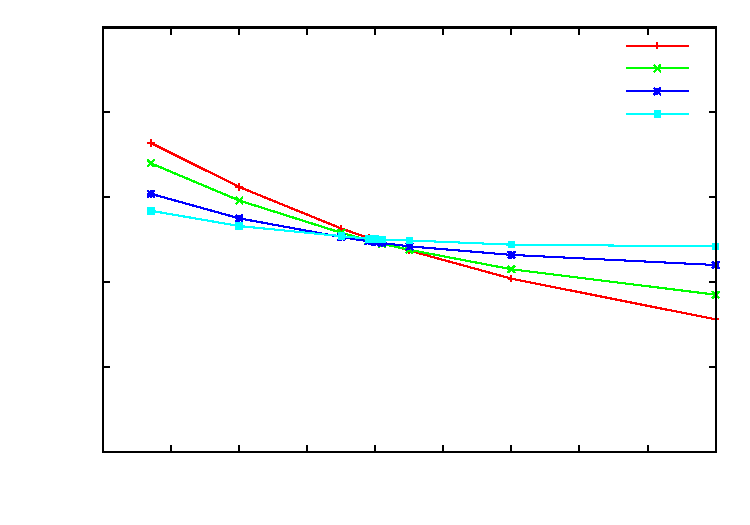
\includegraphics{vary_m}}%
    \gplfronttext
  \end{picture}%
\endgroup

\caption{Plot of reliability index versus the modified section slope for all sections.}
\label{fig:vary_m}
\end{figure}


\clearpage
\section{Discussion}
\subsection{Verification study}
Results of the verification study are given in Figure~\ref{fig:verification_s} and
Figure~\ref{fig:verification_m}.

Verification was performed on results from varying $\bar{S}$ in section~B
and on results from varying $\bar{m}$ in section~D.
These two cases were semi-randomly chosen, while ensuring that different sections 
under variation of different parameters were represented.
The sensitivity behaviour of the reliability index in these two cases 
was also markedly different.

Both verifications showed a good agreement between
reliability index values from FORM and from Monte Carlo simulations with 50 000 trials.

\subsection{Sensitivity of reliability index to variations in $\bar{S}$}
Results from variations in $\bar{S}$ are given in Figure~\ref{fig:vary_s}.

Section slope did not affect the sensitivity behaviour of the reliability
index to variations in $\bar{S}$.
The sentitivity of the reliability index to variations
in $\bar{S}$ was slightly greater at higher $\beta$ values.

\subsection{Sensitivity of reliability index to variations in $\bar{n}$}
Results from variations in $\bar{n}$ are given in Figure~\ref{fig:vary_n}.

Section slope did not affect the sensitivity behaviour of the reliability
index to variations in $\bar{n}$.
The sensitivity of the reliability index was slightly greater at lower $\beta$
values.

\subsection{Sensitivity of reliability index to variations in $\bar{Q}$}
Results from variations in $\bar{Q}$ are given in Figure~\ref{fig:vary_q}.

Section slope did not affect the sensitivity behaviour of the reliability
index to variations in $\bar{Q}$.
The sensitivity of the reliability index was significantly greater at higher $\beta$
values.

\subsection{Sensitivity of reliability index to variations in $\bar{m}$}
Results from variations in section slope are given in Figure~\ref{fig:vary_m}.

Steeper section slopes (lower $m$) resulted in a significantly greater sensitivity of
the reliability index to variations in $\bar{m}$. 
The sensitivity of the reliability index was also significantly 
greater at higher $\beta$ values.

\subsection{General observations}
Generally, the sensitivity of the reliability index was seen to increase
at higher $\beta$ values.
This is significant for civil engineering design, which usually
requires high levels of safety, corresponding to high $\beta$ values.
Only for variations in $\bar{n}$ did the sensititvity of the reliability
index decrease (but only slightly) at higher $\beta$ values.

For most of the parameters investigated, the sensitivity behaviour of 
the reliability index did not differ among the different sections considered.
Only under variations in $\bar{m}$ itself was there a difference
among the different sections considered. 
Checking back with the performance function, this was attributed to
the $(1+m)^{1/8}$ term in the expression for $y$. 

The increasing sensitivity of the reliability index to variations in 
$\bar{Q}$ and $\bar{m}$ at higher reliability index was attributed
to $Q$ and $m$ being present in both terms ($y$ and $y_c$) of the
performance function.


\section{Conclusion}
Sensitivity of the reliability index against initiation of supercritical
flow in triangular channels generally increased at higher $\beta$ values.
This is significant for civil engineering design which usually requires
high $\beta$ values.
The sensitivity behaviour was generally not altered by the section slope of the
triangular channel. 
Results from FORM were found to agree well with results from Monte Carlo
simulations.


\end{document}
